% 2018.01.08 Modified
% 2015.07.10 Modified
%
% mthesis.tex
%
\documentclass[12pt,dvipdfmx]{jarticle} % Japanese
%\documentclass[12pt,dvipdfmx]{article} % English
% if there are problems in the above regarding fonts, use this
%\documentclass[UTF8]{ctexart}

\usepackage[utf8]{inputenc}
%\usepackage{utf}
\usepackage{naist-jmthesis} %Japanese
%\usepackage{naist-mthesis} %English

\usepackage{graphicx}
\usepackage{here}
\usepackage{url}
\usepackage{tabularx}

\usepackage{listings,jvlisting} %日本語のコメントアウトをする場合jvlisting(もしくはjlisting)が必要
%ここからソースコードの表示に関する設定
\lstset{
  basicstyle={\ttfamily},
  identifierstyle={\small},
  commentstyle={\smallitshape},
  keywordstyle={\small\bfseries},
  ndkeywordstyle={\small},
  stringstyle={\small\ttfamily},
  frame={tb},
  breaklines=true,
  columns=[l]{fullflexible},
  numbers=left,
  xrightmargin=0zw,
  xleftmargin=3zw,
  numberstyle={\scriptsize},
  stepnumber=1,
  numbersep=1zw,
  lineskip=-0.5ex
}
%\renewcommand{\lstlistingname}{コマンド}
%
% Page style
%
\pagestyle{final}       % Camera-Ready
%\pagestyle{draft}      % Draft
%
%
\lang{Japanese} % Japanese
%\lang{English} % English
%
% Student Number
%
\studentnumber{1911253}
%
% 修士論文 か 課題研究 かの選択
%
\doctitle{\mastersthesis}       % 修士論文
%\doctitle{\mastersreport}      % 課題研究
%
% 取得予定の修士号は 修士(工学) か 修士(理学) か ?
%
\major{\engineering}    % 工学
%\major{\science}       % 理学
%
% 日本語題目 (in LaTeX)
%
\title{ボランティアコンピューティング資源活用による

クラウドゲーミングのQoE向上に関する研究}
%
% 日本語題目 (in plain text)
%
%   注: (in LaTeX)と同じ場合は指定する必要なし。
%       この情報は修士論文/課題研究には現れませんが、管理のために必要です。
%
\ptitle{太陽と月を利用したpiの低速計算アルゴリズムに関する理論的研究}
%
% 英語題目 (in LaTeX)
%
\etitle{Research on QoE Improvement of Cloud Gaming by Utilizing Volunteer Computing Resources}
%
% 英語題目 (in plain text)
%
%   注: (in LaTeX)と同じ場合は指定する必要なし。
%       この情報は修士論文/課題研究には現れませんが、管理のために必要です。
%
\eptitle{Theoretical Studies on Low-Speed Calculation Algorithms of pi \\
Utilizing the Sun and the Moon}
%
% 日本語氏名 (in LaTeX)
%   (姓と名の間に空白を入れて下さい)
%
\author{前田 健登}
%
% 日本語氏名 (in plain text)
%
%   注: (in LaTeX)と同じ場合は指定する必要なし。
%       この情報は修士論文/課題研究には現れませんが、管理のために必要です。
%
\pauthor{}
%
% 欧文氏名 (in LaTeX)
%   (first name, last name の順に記入し、先頭文字のみを大文字にする。)
%
\eauthor{Kento Maeda}
% 別の例: \eauthor{Kurt G\"{o}del}
%
%
% 欧文氏名 (in plain text)
%
%   注: (in LaTeX)と同じ場合は指定する必要なし。
%       この情報は修士論文/課題研究には現れませんが、管理のために必要です。
%
\epauthor{}
% 別の例: \peauthor{Kurt Goedel}
%
%
% 論文提出年月日
%
\syear{2021}
\smonth{1}
\sday{25}
%
% 専攻の選択
%
%\department{\infproc}  % 情報処理学
%\department{\infsys}    % 情報システム学
%\department{\bioinf}   % 情報生命科学
\department{\infsci}    % 情報科学
%
%
% 審査委員(日本語)
%   (姓と名、名と称号の間に空白を入れて下さい)
%
%5人以上の場合,5人目以降は\addcmembers を使って宣言する。
%最大で合わせて8人まで宣言可能。
%主指導教員、副指導教員を明記する。両指導教員以外は委員。
%学外審査委員は、大学名を明記する
%
% 4人の場合
\cmembers{飯田 元 教授}{(主指導教員)}
         {藤川 和利 教授}{(副指導教員)}
         {市川 昊平 准教授}{(副指導教員)}
         {高橋 慧智 助教}{(副指導教員)}
%
% 3人の場合
%\cmembers{○○ ○○ 教授}{(主指導教員)}
%         {○○ ○○ 教授}{(副指導教員)}
%         {○○ ○○ 准教授}{(副指導教員)}
%         {}{}
%
% 2人の場合
%\cmembers{○○ ○○ 教授}{(主指導教員)}
%         {○○ ○○ 教授}{(副指導教員)}
%          {}{}
%          {}{}
%
% 5人目の宣言
%\addcmembers{55 55 准教授}{(□□大学)}
%            {}{}
%            {}{}
%            {}{}
%
% 5〜6人目の宣言
%\addcmembers{55 55 准教授}{(□□大学)}
%            {66 66 准教授}{(□□大学)}
%            {}{}
%            {}{}
%
% 5〜7人目の宣言
%\addcmembers{55 55 准教授}{(□□大学)}
%            {66 66 准教授}{(□□大学)}
%            {77 77 准教授}{(□□大学)}
%            {}{}
%
% 5〜8人目の宣言
%\addcmembers{55 55 准教授}{(□□大学)}
%            {66 66 准教授}{(□□大学)}
%            {77 77 准教授}{(□□大学)}
%            {88 88 准教授}{(□□大学)}
%
%
% 審査委員(英語)
%     (first name, last name の順に記入し、先頭文字のみを大文字にする。
%       first name と last name の間に空白、
%       last name と 称号の間にカンマと空白を入れて下さい。)
%
% 5人以上の場合,5人目以降は\eaddcmembers を使って宣言する
% Supervisor, Co-supervisor, and Member must be specified.
% 4人の場合
\ecmembers{Professor Hajimu Iida}{(Supervisor)}
          {Professor Kazutoshi Fujikawa}{(Co-supervisor)}
          {Associate Professor Kouhei Ichikawa}{(Co-supervisor)}
          {Assistant Professor Keichi Takahashi}{(Co-supervisor)}
%
% 3人の場合
%\ecmembers{Professor XXX XXX}{(Supervisor)}
%          {Professor XXX XXX}{(Co-supervisor)}
%          {Associate Professor XXX XXX}{(Co-supervisor)}
%          {}{}
%
% 2人の場合
% \ecmembers{Professor XXX XXX}{(Supervisor)}
%           {Professor XXX XXX}{(Co-supervisor)}
%           {}{}
%           {}{}
%
% 5人目の宣言
%\eaddcmembers{Professor 55 55}{(YY University)}
%            {}{}
%            {}{}
%            {}{}
%
% 5〜6人目の宣言
%\eaddcmembers{Professor 55 55}{(YY University)}
%             {Professor 66 66}{(YY University)}
%             {}{}
%             {}{}
%
% 5〜7人目の宣言
%\eaddcmembers{Professor 55 55}{(YY University)}
%             {Professor 66 66}{(YY University)}
%             {Professor 77 77}{(YY University)}
%             {}{}
%
% 5〜8人目の宣言
%\eaddcmembers{Professor 55 55}{(YY University)}
%             {Professor 66 66}{(YY University)}
%             {Professor 77 77}{(YY University)}
%             {Professor 88 88}{(YY University)}
%
%
%
% キーワード5〜6個 (in LaTeX)
%
\keywords{ネットワーク,クラウド,クラウドゲーミング,ボランティアコンピューティング}
%
% キーワード5〜6個 (in plain text)
%
%   注: (in LaTeX)と同じ場合は記入する必要なし。
%       この情報は修士論文/課題研究には現れませんが、管理のために必要です。
%
\pkeywords{pi, 天文学, 数学, 計算機, アルゴリズム}
%
% 5 or 6 Keywords (in LaTeX)
%
\ekeywords{network, cloud, cloud gaming, volunteer computing}
%
% 5 or 6 Keywords (in plain text)
%
%   注: (in LaTeX)と同じ場合は記入する必要なし。
%       この情報は修士論文/課題研究には現れませんが、管理のために必要です。
%
\epkeywords{pi, astronomy, mathematics, computer, algorithm}
%
% 内容梗概 (in LaTeX)
%
%   注: 行の先頭が\\で始まらないようにすること。
%
\abstract{
人類がこの地上に現われて以来、$\pi$の計算には多くの関心が払われてきた。

本論文では、太陽と月を利用して$\pi$を低速に計算するための
画期的なアルゴリズムを与える。

ここには内容梗概を書く。ここには内容梗概を書く。ここには内容梗概を書く。
ここには内容梗概を書く。ここには内容梗概を書く。ここには内容梗概を書く。
ここには内容梗概を書く。ここには内容梗概を書く。ここには内容梗概を書く。
ここには内容梗概を書く。ここには内容梗概を書く。ここには内容梗概を書く。
ここには内容梗概を書く。ここには内容梗概を書く。ここには内容梗概を書く。

ここには内容梗概を書く。ここには内容梗概を書く。ここには内容梗概を書く。
ここには内容梗概を書く。ここには内容梗概を書く。ここには内容梗概を書く。
ここには内容梗概を書く。ここには内容梗概を書く。ここには内容梗概を書く。
ここには内容梗概を書く。ここには内容梗概を書く。ここには内容梗概を書く。
ここには内容梗概を書く。ここには内容梗概を書く。ここには内容梗概を書く。
}
%
% 内容梗概 (in plain text)
%
%   注: (in LaTeX)と同じ場合は記入する必要なし。
%       この情報は修士論文/課題研究には現れませんが、管理のために必要です。
%       改行する箇所には空白行を入れる。
%       行の先頭が\\で始まらないようにすること。
%
\pabstract{
人類がこの地上に現われて以来、piの計算には多くの関心が払われてきた。

本論文では、太陽と月を利用してpiを低速に計算するための
画期的なアルゴリズムを与える。
}
%
% Abstract (in LaTeX)
%
%  注:  行の先頭が\\で始まらないようにすること。
%
\eabstract{
    Cloud gaming, which runs games on cloud servers instead of player-owned gaming
    consoles or PCs, has been attracting much attention from the gaming industry.
    Since a player's device only receives the game screen streamed from the cloud
    server, even poorly performing mobile devices such as smartphones or tablets
    can provide a high-quality gaming experience. However, cloud gaming suffers
    from high response delay (duration between the player's input and when the
    input is reflected on the screen). The breakdown of the response delay
    includes the rendering time, video encoding/decoding time, and network delay
    between the player's device and the cloud server, but recent studies have
    shown that network delay is most significant. Therefore, reducing the network
    delay is crucial to improve the Quality of Experience (QoE) of cloud gaming.
    In this thesis, I propose a system that reduces the network latency by
    applying volunteer computing, a concept where computation is distributed
    across a large number of computing resources contributed by volunteers, and by
    running the cloud game server on a computer geographically close to the
    player. I implemented a prototype of the proposed system and evaluated the
    communication performance and the frame rate during gameplay to quantify the
    QoE. The results reveal the conditions where the proposed system provides
    better QoE than conventional cloud gaming systems and demonstrates that the
    proposed system does not degrade the QoE of gameplay.
}
%
% Abstract (in plain text)
%
%   注: (in LaTeX)と同じ場合は記入する必要なし。
%       この情報は修士論文/課題研究には現れませんが、管理のために必要です。
%       改行する箇所には空白行を入れる。
%       行の先頭が\\で始まらないようにすること。
%
\epabstract{
The calculation of pi has been paid much attention since human beings
appeared on the earth.

This thesis presents novel low-speed algorithms to calculate
pi utilizing the sun and the moon.
}
%%%%%%%%%%%%%%%%%%%%%%%%% document starts here %%%%%%%%%%%%%%%%%%%%%%%%%%%%
\begin{document}
%
% 表紙 および アブストラクト
%
\titlepage
\cmemberspage
\firstabstract
\secondabstract
%
% 目次
%
\toc
\clearpage
\listoffigures
%\newpage
\listoftables
%
% これ以降本文
%
\clearpage
\pagenumbering{arabic}
\section{はじめに}
ゲーム産業は娯楽産業の中でも大きな収益を上げている産業であり、2019年の世界ゲームコンテンツ市場の規模は15兆6898億円と推定されている\cite{prtimes}。国内でも10年連続で成長しており、市場規模は1兆7330億円となっている。その中でも家庭用ハードや家庭用ソフトと比較して、スマートフォンのアプリやPC向けのオンラインゲームなどといったオンラインプラットフォームのゲームの市場規模が年々大きく拡大している。このようにゲームのプレイスタイルがゲーム専用のハードを購入するというものから汎用デバイスでのゲームプレイへと変化を見せている。こういった状況下で注目されている新たな手法で展開されるゲームサービスの一つにクラウドゲーミングがある。

従来のゲームプレイは、プレイヤーがゲーム専用ハードやゲーミングPC等を所有し、その上でゲームを動作させることによって実現されている。一方、クラウドゲーミングというサービスにおいては、図\ref{fig:cloudgaming}のようにクラウドサーバ上でゲームを動作させてその画面をクライアントであるプレイヤーの端末にストリーミングすることで、ゲームをネットワーク越しにプレイすることを可能にしている。このとき、プレイヤーがゲームプレイに使用する端末は、クラウドサーバより送信されるゲーム画面の再生とプレイヤーの操作のサーバへの送信だけを行う。この仕組みによって、スマートフォンやタブレット端末等の性能が貧弱なデバイスでも、従来は高価なゲームハードやゲーミングPCを使用しなければ体験できなかったような高品質なゲーム体験を得られることが期待されている。

\begin{figure*}[t]
    \centering
    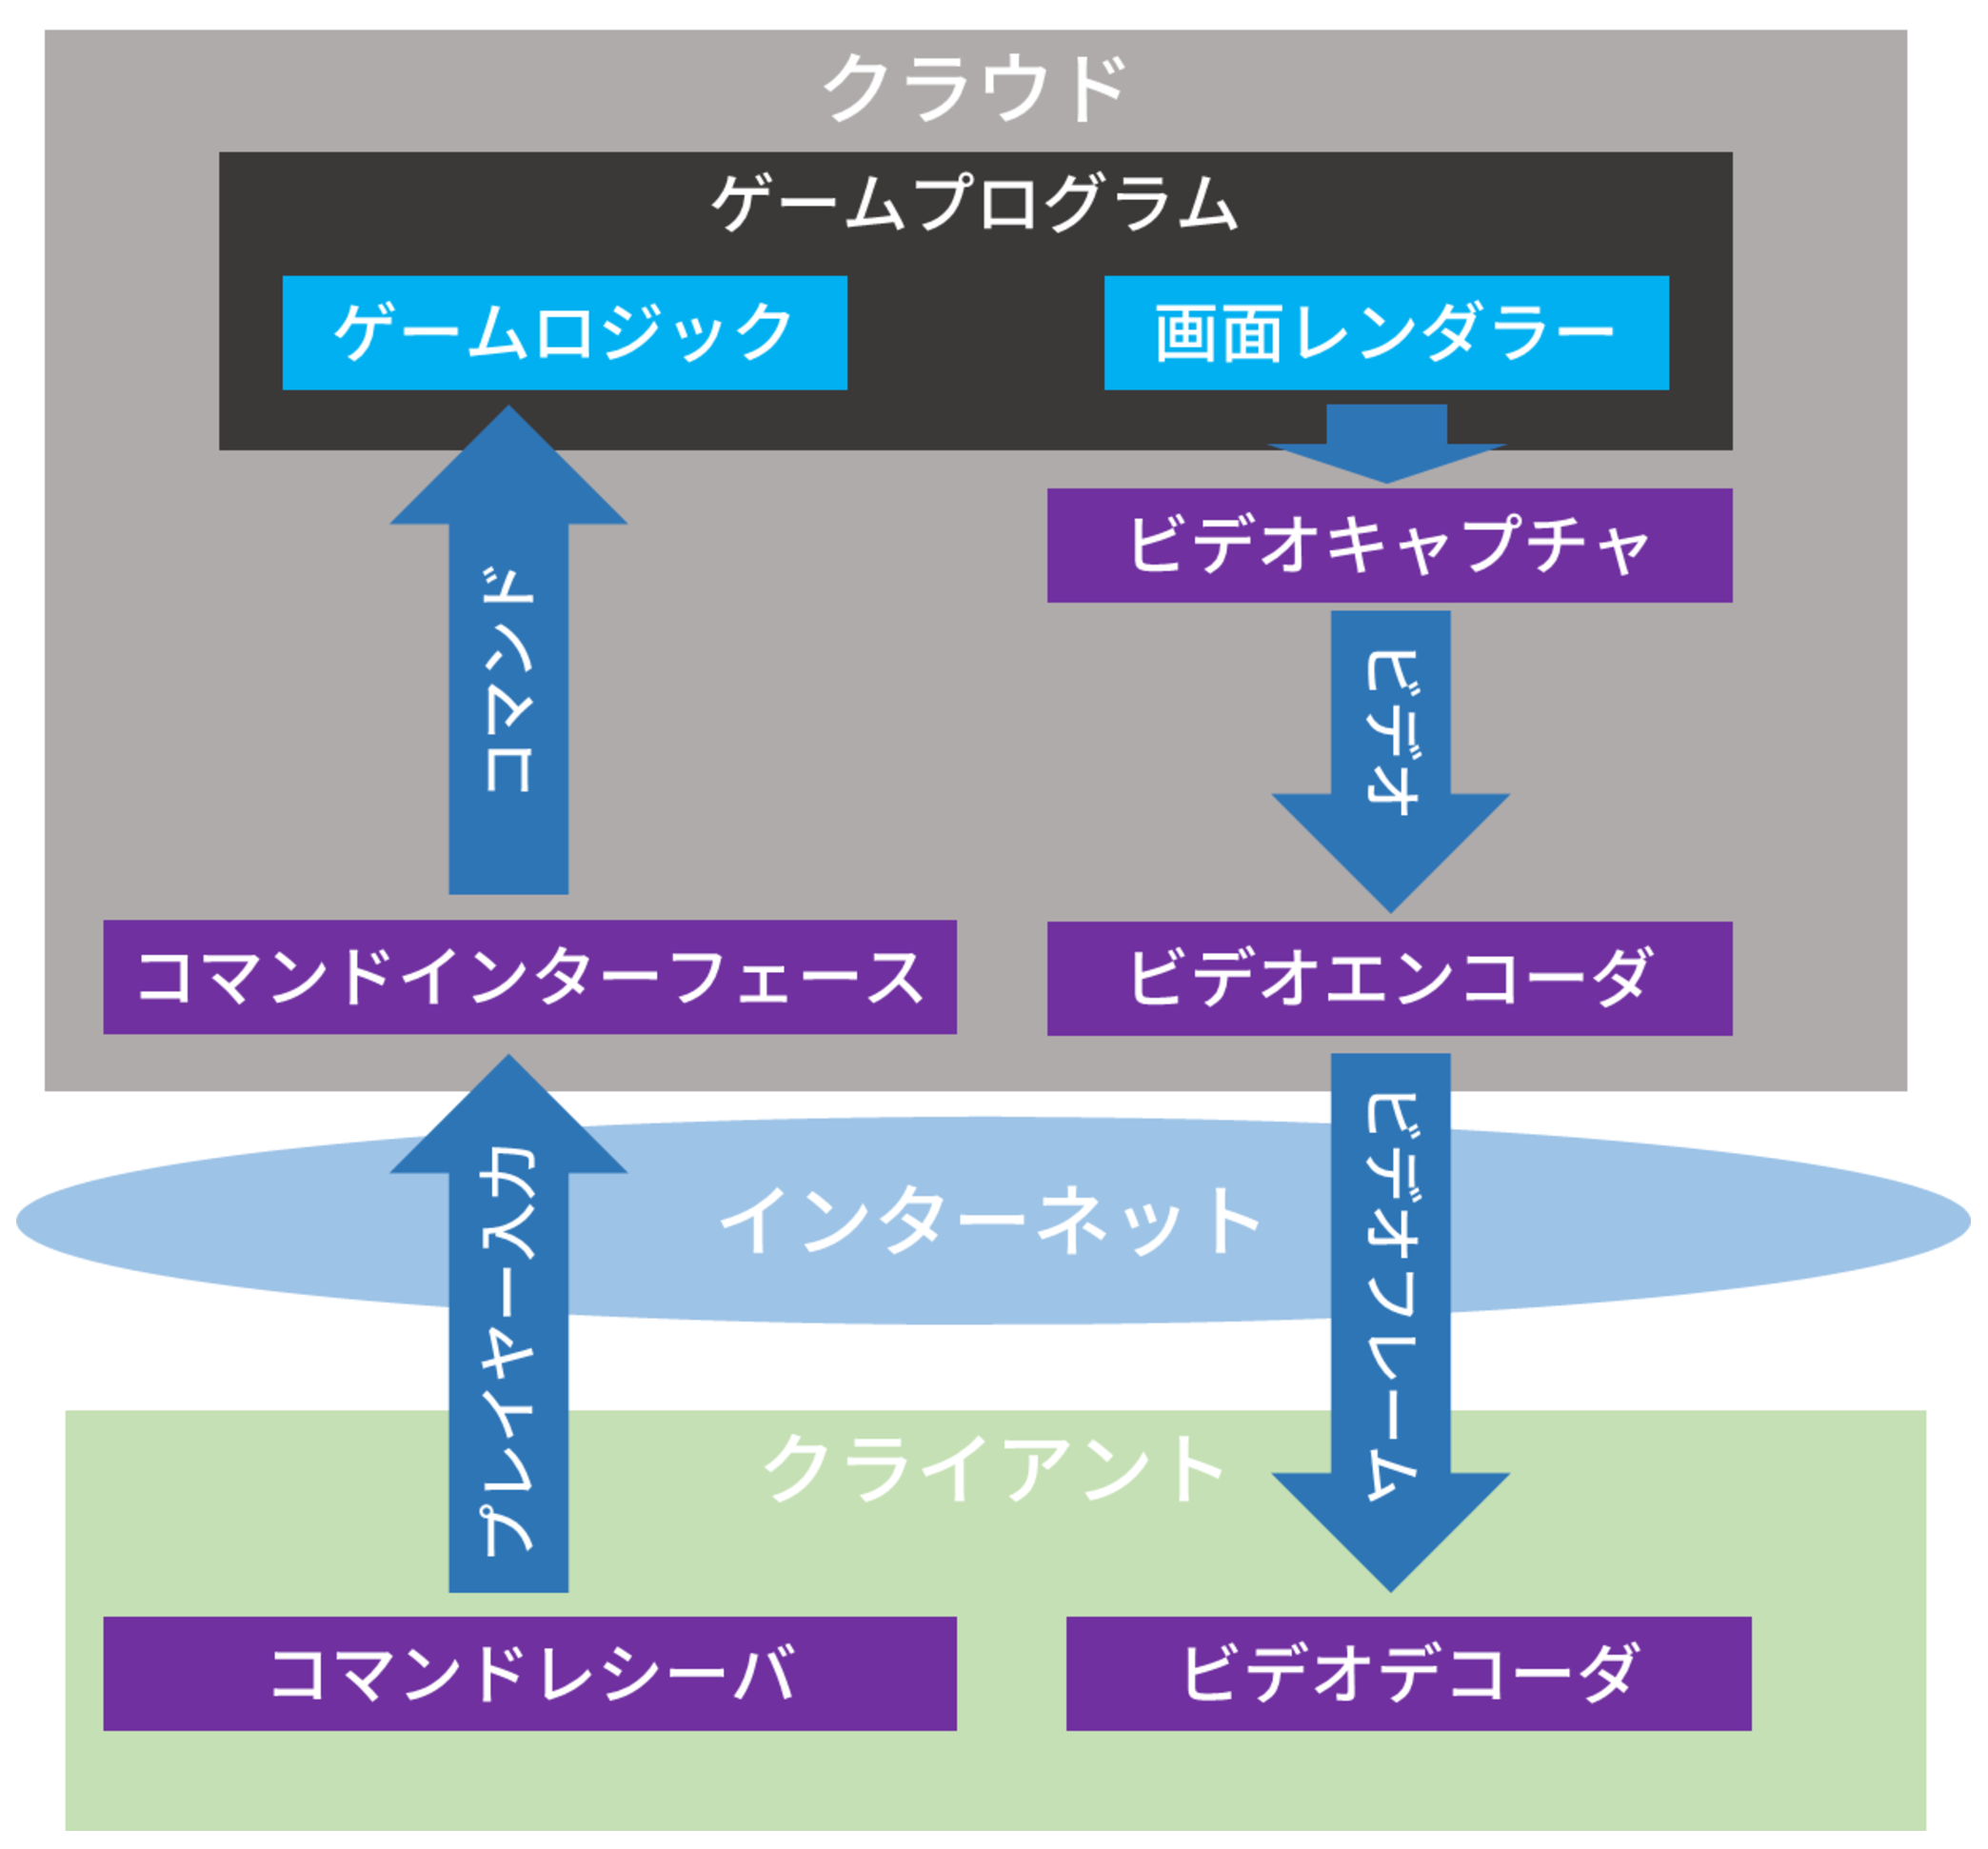
\includegraphics[width=0.8\textwidth,keepaspectratio,clip]{img/cloudgaming.eps}
    \caption{クラウドゲーミングシステム}
    \label{fig:cloudgaming}
\end{figure*}

クラウドゲーミングは商用のサービスの展開もある。過去には英国のOnLive\cite{onlive}やアメリカのGaikaiがクラウドゲーミングサービスを展開していた。これらは既にサービスを終了しているが、ソニーが2012年にGaikaiを買収し、2015年にサービスを閉鎖したOnLiveの資産を取得した\cite{onlive-sony-gaikai}。同年に、ソニーは新たにクラウドゲーミングサービスのPlayStation Now\cite{ps-now}を開始した。また、Googleも2019年にクラウドゲーミングサービスであるGoolge Stadia\cite{stadia}を開始した。同社のウェブブラウザであるGoogle Chromeをインターフェースとしているのが特徴で、ユーザーへのメディアのストリーミングに動画配信サービスのYouTubeを使用している。現在は日本を含まない14カ国で展開されている。また、グラフィックプロセッシングユニットのメーカーとして知られるNVIDIAが提供するクラウドゲーミングサービスGeForce NOW\cite{geforce-now}は、従来PCゲームをプレイしていたプレイヤーをメインターゲットに据えており注目されている。他に、MicrosoftのProject xCloudやAmazonのLunaが海外でサービス開始されている。

商用サービスだけでなく、研究開発用のクラウドゲーミングプラットフォームも存在する。Huangら\cite{gaminganywhere}は、既存のクローズドソースのシステムではクラウドゲーミングを体験するためのテストベッドの設置が困難であることから、オープンソースのクラウドゲーミングプラットフォームであるGamingAnywhereを開発した。GamingAnywhereはWindows、Linux、OS X上で実装されており、クライアントはiOSやAndroid等の他のOSにも移植が可能である。また、GamingAnywhereは詳細な設定を可能にしていて、更にオープンソースであるため拡張的な実装が可能であるなど、クラウドゲーミングのシステム研究のテストベッドの構築に適している。

従来のゲームシステムとは一線を画するクラウドゲーミングには、依然として重要な課題が存在している\cite{cloudgaming-survey}。クラウドゲーミングプロバイダの立場から見た課題としては、ゲーム環境の仮想化やサーバにおける負荷分散などといった課題がある。一方、システムのユーザーであるプレイヤーが知覚するゲーム体験の品質の評価指標であるQuality of Experience(QoE)
を確保することも重要な課題である。クラウドゲーミングのプレイにおけるQoEの確保に必要な課題の構成要素としては、以下のようなものがある。
\begin{itemize}
    \item ストリーミングされるゲーム画面の高品質な画質の担保
    \item ゲーム画面のリアルタイムストリーミングに耐えうる、充分なネットワーク帯域の確保
    \item 伝送データ圧縮や効率的なストリーミング技術
    \item プレイヤー端末での画面表示やプレイヤーによる操作が画面に反映されるまでの遅延の最小化
\end{itemize}

中でもプレイヤーの操作に対する応答性に直結する遅延の問題は重要である。動画配信プラットフォームにおけるライブストリーミングの場合、途切れることなく安定した動画の配信を行うためにバッファリングを行うことで対処する場合がある。しかしクラウドゲーミングは多くの場合、リアルタイムかつインタラクティブな性質を持つコンテンツであるためこの方法を使用することができない。そのため、クラウドサーバ上でのゲーム画面生成の高速化/効率化や、伝送データの圧縮、ネットワーク遅延の最小化などが課題となっている。

クラウドのデータセンターは、通常国内には数箇所しか設置されていない。このため、データセンターに地理的に遠いプレイヤーの端末から接続するとネットワーク遅延が大きくなってしまうという問題がある。データセンターに計算機資源を集約する現在のクラウドアーキテクチャを利用する限り、この遅延を解消することはできない。プレイヤーとクラウド上の計算機資源との間の物理的距離に起因する遅延の問題解決するためには、プレイヤーの近傍に計算機資源を設置することが必要である。

ところで、多量のタスクを小規模なタスクに分割して、ボランティアの提供する多数のコンピュータリソースに広域に分散して処理するボランティアコンピューティングという枠組みがある。SETI@home\cite{setiathome}やFolding@home\cite{folding}に代表されるボランティアコンピューティングプロジェクトが、高エネルギー物理学、分子生物学、医学、天体物理学、気候研究などの分野の研究で利用された。クラウドコンピューティングの枠組みにおいては、クラウドサーバに一極集中したリソースにユーザがアクセスして利用する。それに対し、ボランティアコンピューティングにおいては、広域に分散した一般ユーザーのリソースを活用するという特徴がある。国内に数箇所しか設置されていないクラウドのデータセンターに比べて、広域に分散した一般ユーザーのリソースは地理的に近傍である可能性が高い。この性質を利用し、よりネットワーク遅延の小さい計算機同士での通信でクラウドゲーミングを行えば、遅延の問題を解消する可能性がある。

本研究では、ボランティアが提供する地理的に近傍の遊休コンピュータのリソースを活用することによるクラウドゲーミングシステムを提案する。既存のクラウドゲーミングアーキテクチャにおいては、クラウドのデータセンターでゲームが動作しているために、プレイヤーの端末からデータセンターまでのネットワーク遅延を回避することは不可能である。国内のデータセンターまでのネットワーク遅延は最大50ms程度と言われている(出典がない)。これはゲームプレイにおけるレスポンスの遅延としては無視できない値であり、著しくプレイヤーのQoE低下の原因となり得る。本研究では、プレイヤーの端末からデータセンターまでのネットワーク遅延を削減し、プレイヤーがクラウドゲーミングのプレイを通して体験する画面表示や操作の反映の遅延を最小化することでのプレイヤーのQoEの向上を目的とする。広域に分散したボランティアの提供する遊休コンピュータの中から、プレイヤーの端末から見て地理的に近傍のものを選択し、その上でクラウドゲームサーバを動作させる。これによって遅延の削減を目指す。

本論文の以後の部分は次のように構成されている。2章では、研究分野の背景、関連研究について述べる。3章では、提案システムの設計について述べる。4章では、提案システムの実装について述べる。5章では、提案システムの性能評価について述べる。6章では、まとめと今後の展望について述べる。







 


\clearpage
\section{背景}
本章では、研究の背景および既存の研究について述べる。

\subsection{クラウドゲーミング}
クラウドゲーミングシステムはOnLiveやGaikaiといった商用サービスから始まったが、それらのクローズドシステムではゲームプレイ体験や可用性、スケーラビリティといった要素のテストベッドとして活用することは困難である。Huangら\cite{gaminganywhere}は、研究開発に利用できる高い拡張性、移植性を備えたオープンソースのクラウドゲーミングプラットフォームであるGamingAnywhereを開発した。GamingAnywhereは以下の3つの設計目標に沿って設計されている。
\begin{itemize}
    \item オープンソースのシステムであり、ビデオストリーミングなどのコンポーネントを、異なるアルゴリズムや規格、プロコトルで実装した別のコンポーネントに容易に置き換えが可能である
    \item クロスプラットフォームであり、Windows、Linux、OS Xで利用可能である
    \item メモリコピー回数を減らす等の時間的/空間的なオーバーヘッドを最小化し、効率的に動作する
\end{itemize}
GamingAnywhereはこれらの実験を通して実装された。大規模な実験を通して商用クラウドゲーミングシステムであるOnLiveとStreamMyGameを大幅に凌駕することが示された。StreamMyGameは、Windows向けのゲームおよびアプリケーションに対し、WindowsおよびLinuxの端末でのリモートプレイを可能にするソフトウェアである。GamingAnywhereと比較すると、OnLiveとStreamMyGameは内部における処理遅延が最大で3倍および10倍になり、またビデオ品質についてはそれぞれ3dbおよび19db低くなるという結果が示されている。また、GamingAnywhereはクラウドゲーム開発者やシステム研究者に公開され、クラウドゲーミングシステムのテストベッドとして使用することができる。

Sheaら\cite{cloudperformance}は、OnLiveを対象としてクラウドゲーミングプラットフォームのパフォーマンスを測定した。その結果、ストリーミング品質およびインタラクションの遅延が、クラウドゲーミングを構成するゲーム、計算機、ネットワークのすべての部分で課題を抱えていることを指摘した。また、携帯電話のネットワークにおいて200msを超えるネットワーク遅延の回線は珍しくなく、これにより多くのゲームにおいてインタラクション遅延が高くなりすぎる可能性について指摘した。さらに、ゲーム画面のレンダリングとゲームロジックの一部をプレイヤー端末のローカルで実行することにより、インタラクションの遅延などのクラウドゲーミングの課題の一部を隠蔽するシステムの可能性についても言及している。

クラウドゲーミングが抱える遅延の課題について、Leeら\cite{outatime}は、将来起こりうる画面フレームを投機的にレンダリングするOutatimeを提案した。Outatimeは以下の処理を組み合わせて構成されている。
\begin{itemize}
    \item 将来のゲームの状態予測
    \item 画像ベースレンダリングとゲームイベントのタイムシフトによる状態近似
    \item チェックポイントとロールバックの機構による予測の誤りが前方に伝播することの防止
    \item 帯域幅の節約のための状態圧縮
\end{itemize}
投機的にレンダリングされた画面フレームは一つのRTTに事前にプレイヤーの端末に配信され、予測と異なる状態に遷移した際に迅速に回復する。これにより、クラウドゲーミングで発生するネットワーク遅延を最大120ms隠蔽できると述べている。一方で、ゲームのステージ内をワームホールでテレポートするようなイベントについては、この手法では対応できないということも指摘している。

クラウドゲーミングで発生する遅延のうちでも大きな要因であるネットワーク遅延の課題に対し、Hongら\cite{placing}はクラウドゲームサーバとして動作するVM配置の最適化によって解決を試みた。プレイヤーのQoEとプロバイダの純利益との間のトレードオフであるクラウドゲーミングの最適化を行うためのヒューリスティックアルゴリズムを開発した。この中で、クラウドゲームサーバの役割を果たすVMを、プレイヤーの端末から最もネットワーク遅延が小さい位置にあるサーバに割り当てるという最適化を行っている。また、開発したアルゴリズムを評価するために大規模なシミュレーションを実施しており、結果としてアルゴリズムが以下のことを示している。
\begin{itemize}
    \item 最適に近いソリューションが得られる
    \item 20000台のサーバと40000人のプレイヤーを抱える大規模なクラウドゲーミングサービスへの拡張が可能である
    \item 最先端の既存ヒューリスティックアルゴリズムを上回る結果が得られること
\end{itemize}
一方、この手法においてもプレイヤー端末からデータセンターまでのネットワーク遅延を回避できないという課題の解決には至っていない。


\subsection{ボランティアコンピューティング}
ボランティアコンピューティングは多量のタスクを小規模なタスクに分割して、ボランティアの提供する多数のコンピューティングリソースに分散して処理する枠組みである。ボランティアのリソースで動作するクライアントは、定期的にサーバと通信を行い、完了したタスクの報告と新しいタスクの取得を行う。サーバがタスクをディスパッチする速度によって、ボランティアコンピューティングプロジェクトで使用できる計算能力が制限される可能性がある。Andersonら\cite{boinc}は、ボランティアコンピューティング用のミドルウェアシステムであるBerkeley Open Infrastructure for Network Computing (BOINC) を開発した。BOINCのタスクサーバの様々なコンポーネントが使用するCPU時間とディスク帯域幅の測定が行われ、BOINCは1日に8880万個のタスクをディスパッチできると結論付けられた。各クライアントが1日に1つのタスクを発行し、各タスクが1GFLOPSのコンピュータで12時間CPUを使用する場合、ボランティアコンピューティングプロジェクトが880万のクライアントをサポートし、4.4PetaFLOPSの計算能力を得ることができると述べられている。

ボランティアコンピューティングは、前述のように本来は科学技術計算を膨大な数の一般ユーザの計算機資源を用いて分散処理する仕組みを提供するものである。しかし、多数の一般ユーザの計算機資源を利用している点に注目すると、中央集権的なクラウドコンピューティングのアーキテクチャと異なり、エンドユーザに地理的に近傍に利用可能な計算機環境を広く配備することが可能なプラットフォームと考えられる。このような広域分散システムの活用により、既存のクラウドゲーミングが抱える遅延の課題を解決できる可能性がある。ただし、既存のボランティアコンピューティングにおいて、ボランティアが提供する計算機ノードは基本的にタスク配信を行う中央サーバのみと通信を行い、計算機ノード間で直接通信を行う仕組みはない。ボランティアコンピューティングを物理的に近傍な計算機資源を利用する仕組みとしてクラウドゲーミングに応用する際には、この課題を解決する必要があると考えられる。


\clearpage
\section{設計}
\pagenumbering{arabic}

プレイヤーのPCから最も近い利用可能な遊休コンピュータを探し、クラウドゲームサーバをホストさせるシステム

\subsection{提案システムの概要}
提案システムの概要を図\ref{fig:arch}に示す。
プレイヤーPC上のVCクライアントエージェントがクラウド上のVCコントローラにゲームプレイをリクエスト。VCコントローラが遊休コンピュータにVCホストエージェントにクラウドゲームのホスティングをリクエスト。遊休コンピュータでクラウドゲームサーバとゲームが起動し、プレイヤーPC上のクラウドゲームクライアントと通信してゲームをする。

\subsection{VCコントローラ}
クラウド上に存在するVCコントローラはゲームをプレイしたいプレイヤーのPCと利用可能な遊休コンピュータをマッチングする役割を果たす。プレイヤーPCからのゲームプレイのリクエストを受け取ると、利用可能な遊休コンピュータ群の中からプレイヤーPCからのネットワーク遅延が小さいものを見つける。そしてその遊休コンピュータに対してクラウドゲームのホスティングをリクエストする。また、このマッチングの成立後、VCコントローラはVCクライアントエージェントとVCホストエージェントにクラウドゲームサーバ/クライアントが通信するためのリンクを張るのに必要な情報を配布する。

\subsection{VCクライアントエージェント}
VCクライアントエージェントはボランティアクラウドゲーミングコントローラ上のVCコントローラへゲームプレイのリクエストを送信する。このときプレイしたいゲームやサーバとリンクを張るために必要なネットワーク情報などを付帯して送信する。

\subsection{VCホストエージェント}
VCコントローラに割り当てられた遊休コンピュータ上のVCホストエージェントはクラウドゲームのホスティングのリクエストを受け取る。その後クラウドゲームサーバとゲームを起動し、接続に必要な情報と共にVCクライアントエージェントに起動完了のメッセージを送信する。

\subsection{クラウドゲームサーバ/クライアント}
クラウドゲームサーバはゲーム画面をキャプチャして、ビデオストリームとしてクラウドゲームクライアントに送信する。一方で、クラウドゲームクライアントは受け取ったゲーム画面の描画を行う。また、クラウドゲームクライアントはプレイヤーの入力操作をキャプチャしてクラウドゲームサーバ上のゲームの入力となるように送信を行う。

\begin{figure*}[t]
    \centering
    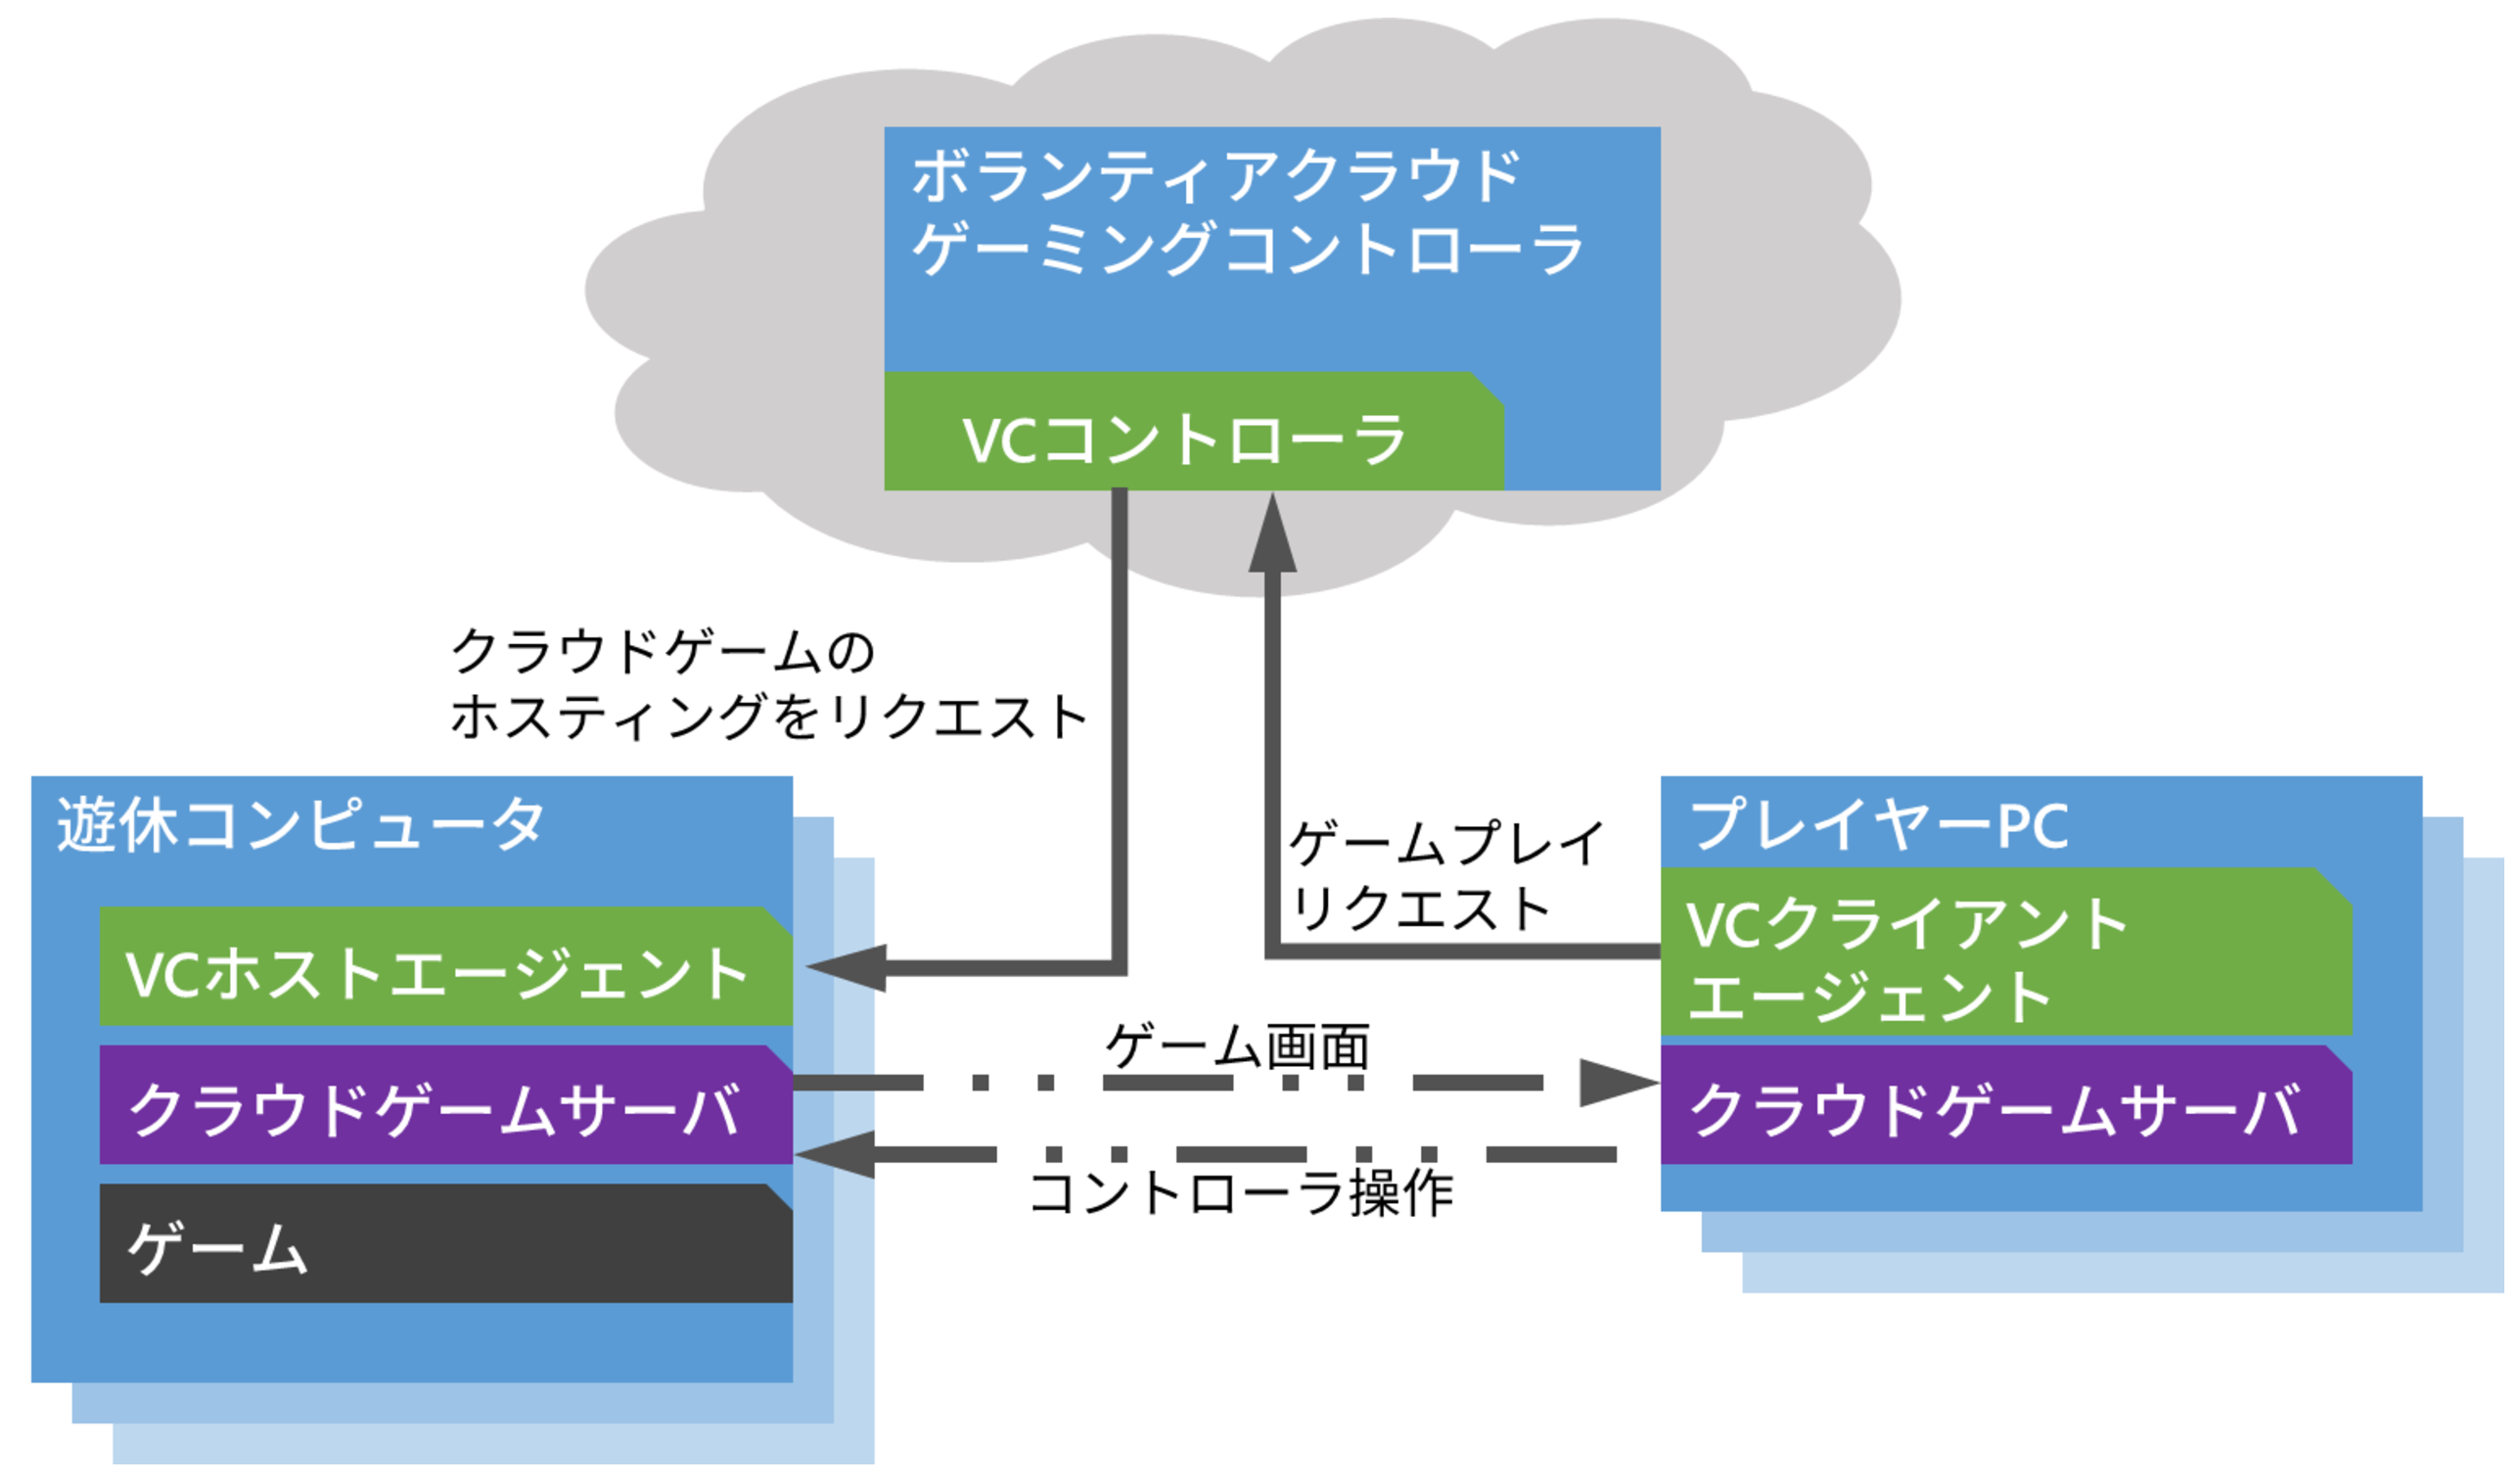
\includegraphics[width=0.8\textwidth,keepaspectratio,clip]{img/architecture.eps}
    \caption{アーキテクチャ}
    \label{fig:arch}
\end{figure*}


\clearpage
\section{実装}
\pagenumbering{arabic}

現在の提案システムの実装はサーバマシンとクライアントマシンがXMPPサーバから取得した情報をもとに直接リンクを張ってクラウドゲーミング通信を展開する方式になっている。クラウドゲームサーバ/クライアントにはオープンソースクラウドゲーミングプラットフォームであるGamingAnywhereを使用している。また、パブリッククラウド等で展開しているサービスではなく、一般のユーザコンピュータでサービスを展開する手法特有の課題とその対処についても本章で述べる。

\subsection{実装上の課題}
パブリッククラウドやビジネス向けのサーバでサービスを展開する場合と異なり、提案システムはクラウドゲームサーバをボランティアの提供するユーザコンピュータ上で展開する。通常ユーザコンピュータはNATやファイアウォールの背後にあり、また固定IPアドレスを持っていないことも多いため直接通信することが難しい。これにより提案システムが必要とする通信において、大きく2つ問題が生じる箇所が出てくる。一つはクラウド上のコントローラから遊休コンピュータへクラウドゲームのホスティング等の直接命令を送ることができないということである。もう一つは、クラウドゲームサーバ/クライアントを展開する遊休コンピュータとプレイヤーPC間での通信において、双方向的な直接通信を展開できないという点である。

\subsection{VCコントローラとエージェントの連携}
VCコントローラと遊休コンピュータ上で動作するVCホストエージェントとの通信の課題についてはgRPC\cite{grpc}を用いる。gRPCはGoogleが開発しているオープンソースのRPCサービスで、異なるコンピュータ間あるいはマイクロサービス間で情報をやり取りするのに使われる。gRPCではクライアントアプリケーションがローカルオブジェクトであるかのようにサーバアプリケーションのメソッドを直接呼び出すことができるため、分散アプリケーション等の実装に適している。サーバ側ではサービスを定義してそのインターフェースを実装する。クライアント側ではサーバと同じメソッドを提供するスタブを介してサーバアプリケーションの機能を使えるようにしているのが特徴である。

gRPCのResponse Streaming gRPCという機能は、単一のリクエストに対して複数のレスポンスを返すことが可能である。これを使用することで、VCクライアントが送信した単一のゲームプレイリクエストに対して、ACKや起動報告、ホスティング終了時の完了報告、エラーの通知など様々なレスポンスを返すことができる。

\subsection{クラウドゲームサーバ/クライアント間のP2P通信}

GamingAnywhere
クラウドゲームサーバとクラウドゲームクライアントとしてGamingAnywhereを使用する

EdgeVPN
\cite{edgevpn}

St Justeら\cite{tincan}が開発した
P2P型のオーバーレイネットワークツール。ネットワークのユーザ/グループ管理が可能。TinCanの論文引用して紹介する。

\subsection{システム動作}



\clearpage
\section{分析}
\pagenumbering{arabic}

\subsection{リンクに対する生の遅延の大小の影響}
tcを使って任意に遅延を挿入し、pingの値で遅延の増え方に影響がないか見る。
遅延が増えたときの遅延の増え方が線形みたいなことを言う。
遅延が増えたときの帯域の減り方の話をする。

\subsection{リンクに対する遅延の大小の帯域への影響}
tcを使って任意に遅延を挿入し、iperfで帯域の減り方への影響を見る
遅延が増えたときの帯域の減り方の話をする。

\subsection{ネットワーク帯域の大小の影響}
tcを使って帯域に制限をかけて、実際に複数のゲームをプレイしたときのフレームレートへの影響を見る。
使用したゲームはSteamで公開されているAlbion Online(MMORPG)、Red Eclipse 2(FPS, Action)、Simply Chess(Board Game)


\clearpage
\section{まとめと今後の課題}
本研究では、ボランティアが研究する地理的に近傍の遊休コンピュータのリソースを活用することによるクラウドゲーミングシステムを提案した。既存のクラウドゲーミングアーキテクチャにおいて、プレイヤーの端末からデータセンターへ接続する際のネットワーク遅延を回避することはできない。この課題を解決するため、広域に分散したボランティアの計算機資源でクラウドゲームサーバをホストするシステムを考案した。実験を通して、提案システムはクラウドゲーミングのプレイにおいてネットワーク遅延やスループットが許容量に収まることを示した。また、ゲームプレイ中のフレームレートについて、低スループットのネットワークを使用した際でも低下が見られないことを示した。これにより、提案システムがクラウドゲーミングのプレイにおけるQoEを低下させることなくサービスを提供できることを示した。

今後の展望としては、利用可能な遊休コンピュータの中から、プレイヤーPCからのネットワーク遅延が小さいものを探索する機能を持つボランティアクラウドゲーミングコントローラの実装を検討している。また、今回の実験は遊休コンピュータとプレイヤーPCがそれぞれ1台ずつの構成で行ったが、これらの数を増やした上でのシステムの負荷試験についても検討する。%この際、ゲームのジャンル毎に許容遅延などのQoEの許容範囲を考慮し、それぞれについて遊休コンピュータのマッチングを調整する必要が考えられる。
この際、ゲーム毎にレンダリングに必要な時間に違いがある可能性についても考慮する必要が考えられる。高画質かつ高フレームレートのゲームなどのレンダリングやエンコードの負荷が大きいゲームの場合、総応答遅延が長くなる。これは相対的にネットワーク遅延が小さくなることを意味する。このとき、提案システムでQoEを維持するために、より近傍の遊休コンピュータを使用して総応答遅延を削減する必要が想定される。
また、ゲームの種類によって許容される応答遅延に差がある可能性についても考慮が必要である。FPSのような低遅延が求められる対戦形式のゲームにおいては、遊休コンピュータのマッチングにおいてプレイヤー端末から最も近傍であることを優先しなければならない可能性がある。一方で、操作や対戦相手の行動が画面に反映されるまでにある程度の遅延が許容されるボードゲームのようなジャンルにおいては、マッチングにおいて近傍であることの優先度を下げるということも考えられる。



%
% 謝辞
%
\clearpage
\acknowledgements
本論文の執筆を進めるに当たり、多くの方々に御指導、御協力を賜りました。ここに御名前を記すと共に、深く感謝の意を示します。

主指導教員であり、本論文の審査委員を務めていただいた、奈良先端科学技術大学院大学 情報科学研究科 飯田 元 教授には、研究の進め方を始めとして、研究の捉え方等、あらゆる面で非常に多くの御指導・御助言を賜りました。心より感謝を申し上げます。

副指導教員であり、本論文の審査委員を務めていただいた、奈良先端科学技術大学院大学 情報科学研究科 藤川 和利 教授には、本研究の扱うべき課題や方針について非常に貴重な御意見を賜り、本研究の方向性を定めていく上で非常に大きな助けとなりました。心より感謝を申し上げます。

副指導教員であり、本論文の審査委員を務めていただいた、奈良先端科学技術大学院大学 情報科学研究科 市川 昊平 准教授には、本研究の立ち上げから提案手法の立案、論文執筆に至るまで、様々な面で研究に関する御指導・御協力を賜りました。心より感謝を申し上げます。

副指導教員であり、本論文の審査委員を務めていただいた、奈良先端科学技術大学院大学 情報科学研究科 高橋 慧智 助教には、研究の方針や提案システムの実装・評価など様々な面で御指導・御協力を賜りました。心より感謝を申し上げます。

奈良先端科学技術大学院大学 情報科学研究科 ソフトウェア設計学研究室秘書の小川 暁子氏には、学生生活やTA/RA業務における書類作成や諸連絡等、事務処理において多大なる御協力を頂きました。心より感謝を申し上げます。

奈良先端科学技術大学院大学 情報科学研究科 ソフトウェア設計学研究室元秘書の仲田 綾奈氏には、学生生活やTA/RA業務における書類作成や諸連絡等、事務処理において多大なる御協力を頂きました。心より感謝を申し上げます。

奈良先端科学技術大学院大学 情報科学研究科 ソフトウェア設計学研究室の諸先輩方、同期生、後輩の皆様には、学生生活において公私共に様々に御助力を頂き有意義な2年間を過ごすことができました。心より感謝を申し上げます。

LIPPS梅田ロフトのスタッフの皆様には、学生生活を送る上で自身を持てる容姿を保つために多大なる尽力を頂きました。心より感謝を申し上げます。
%
% 参考文献
% ここでは \reference を使って、自分でリストを作るか、BibTeX を使って
% リストをつくって下さい。この例では BibTeX を作るような形式になってい
% ます。
%
\clearpage
% \reference
\bibliographystyle{plain}
\bibliography{mthesis}
%
% 付録
%
%\appendix

%\section{おまけその1}
%\label{omake1}

%これはおまけです。これはおまけです。これはおまけです。これはおまけです。


%\section{おまけその2}

%これもおまけです。これもおまけです。これもおまけです。これもおまけです。


\end{document}

